
% \begin{table*}[!t]
% 	\centering
% 	\scriptsize
% 	\caption{Evaluated benchmarks from the PARSEC benchmark suite}
% 	
% 	\setlength{\tabcolsep}{4pt}
% 	\begin{tabular}{|p{1.3cm}|p{6.2cm}|p{2.5cm}|c|c|c|c|}
% 	\hline
% 	\textbf{Benchmark} & \multicolumn{1}{|c|}{\textbf{Description}} & \multicolumn{1}{|c|}{\textbf{Input}} & \textbf{Parallelization} & \textbf{Synchronization} &\multicolumn{1}{|c|}{\textbf{LOC}} &\multicolumn{1}{|c|}{\textbf{Perf ratio}} \\
% 	\hline \hline
% 	blackscholes & Calculates the prices for a portfolio of European options analytically with the Black-Scholes partial differential equation. & 10,000,000 options & data-parallel & dataflow/barrier &404 &2.18 \\ \hline
% 	bodytrack & Computer vision application which tracks a 3D pose of a marker-less human body with multiple cameras through an image sequence. & 4 cameras, 261 frames, 4,000 particles, 5 annealing layers & pipeline & dataflow & 6,968 & 4.16 \\ \hline
% 	canneal & Simulated cache-aware annealing to optimize routing cost of a chip design. & 2.5 million elements, 6,000 temperature steps & unstructured & locks/atomics & 3,040 & 1.73 \\ \hline
% 	dedup & Compresses a data stream with a combination of global compression and local compression in order to achieve high compression ratios. & 351 MB data & pipeline & dataflow/locks & 3,401 & 2.67 \\ \hline
% 	facesim & Takes a model of a human face and a time sequence of muscle activation and computes a visually realistic animation of the modeled face. & 100 frames, 372,126 tetrahedra & data-parallel & dataflow/barrier & 34,134 & 3.40 \\ \hline
% 	ferret & Content-based similarity search of feature-rich data (audio, images, video, 3D shapes, etc.) & 3,500 queries, 59,695 images database, find top 50 images & pipeline & dataflow & 10,552 & 3.59 \\ \hline
% 	fluidanimate & Uses an extension of the Smoothed Particle Hydrodynamics method to simulate an incompressible fluid for interactive animation purposes. & 500 frames, 500,000 particles & data-parallel & dataflow/barrier & 2,348 & 2.64 \\ \hline
% %	freqmine & Intel RMS application which employs an array-based version of the FP-growth (Frequent Pattern-growth) method for Frequent Itemset Mining (FIMI). & 250,000 HTML documents, minimum support 11,000 & 2,231\\ \hline
% %	raytrace & Intel RMS workload which renders an animated 3D scene. & 200 frames, 1,920$\times$1,080 pixels, 10 million polygons & 13,751\\ \hline
% 	streamcluster & Solves the online clustering problem. & 200,000 points per block, 5 block & data-parallel & dataflow/barrier/atomics & 1,769 & 3.48 \\ \hline
% 	swaptions & Intel RMS workload which uses the Heath-Jarrow-Morton (HJM) framework to price a portfolio of swaptions. & 128 swaptions, 1 million  simulations & data-parallel & dataflow/barrier & 1,225 & 2.78 \\ \hline
% %	vips & VASARI Image Processing System (VIPS), which includes fundamental image processing operations. & 18,000$\times$18,000 pixels & 127,957\\ \hline
% %	x264 & H.264/AVC (Advanced Video Coding) video encoder. & 512 frames, 1,920$\times$1,080 pixels & 29,329\\ \hline 
% 	\end{tabular}
% 	\label{tab:parsec}
% 	\vspace{-0.3cm}
% \end{table*}

\begin{table*}[!t]
	\centering
	\scriptsize
	\caption{Benchmarks used from the PARSEC benchmark suite and their 
measured performance ratio between big and little cores}
    %\vspace{-0.2cm}
	\setlength{\tabcolsep}{3pt}
	\begin{tabular}{|p{2cm}|p{4.7cm}|p{2.5cm}|c|c|}
	\hline
	\textbf{Benchmark} & \multicolumn{1}{|c|}{\textbf{Description}} & \multicolumn{1}{|c|}{\textbf{Input}} & \textbf{Parallelization} & \multicolumn{1}{|c|}{\textbf{Perf ratio}} \\
	\hline \hline
	blackscholes & Calculates the prices of a portfolio analytically with the Black-Scholes partial differential equation. & 10,000,000 options & data-parallel &2.18 \\ \hline
	bodytrack & Computer vision application which tracks a 3D pose of a marker-less human body with multiple cameras through an image sequence. & 4 cameras, 261 frames, 4,000 particles, 5 annealing layers & pipeline & 4.16 \\ \hline
	canneal & Simulated cache-aware annealing to optimize routing cost of a chip design. & 2.5 million elements, 6,000 steps & unstructured & 1.73 \\ \hline
	dedup & Compresses a data stream with a combination of global compression and local compression in order to achieve high compression ratios. & 351 MB data & pipeline & 2.67 \\ \hline
	facesim & Takes a model of a human face and a time sequence of muscle activation and computes a visually realistic animation of the modeled face. & 100 frames, 372,126 tetrahedra & data-parallel & 3.40 \\ \hline
	ferret & Content-based similarity search of feature-rich data (audio, images, video, etc.) & 3,500 queries, 59,695 images database, find top 50 images & pipeline & 3.59 \\ \hline
	fluidanimate & Extended Smoothed Particle Hydrodynamics method to simulate an 
incompressible fluid for interactive animations. & 500 frames, 500,000 particles & 
data-parallel & 3.32 \\ \hline
%	freqmine & Intel RMS application which employs an array-based version of the FP-growth (Frequent Pattern-growth) method for Frequent Itemset Mining (FIMI). & 250,000 HTML documents, minimum support 11,000 & 2,231\\ \hline
%	raytrace & Intel RMS workload which renders an animated 3D scene. & 200 frames, 1,920$\times$1,080 pixels, 10 million polygons & 13,751\\ \hline
	streamcluster & Solves the online clustering problem. & 200K points per block, 5 block & 
data-parallel & 3.48 \\ \hline
	swaptions & Intel RMS workload; uses the Heath-Jarrow-Morton framework to price a portfolio of swaptions. & 128 swaptions, 1 million  simulations & data-parallel & 2.78 \\ \hline
%	vips & VASARI Image Processing System (VIPS), which includes fundamental image processing operations. & 18,000$\times$18,000 pixels & 127,957\\ \hline
%	x264 & H.264/AVC (Advanced Video Coding) video encoder. & 512 frames, 1,920$\times$1,080 pixels & 29,329\\ \hline 
	\end{tabular}
	\label{tab:parsec}
	%\vspace{-0.3cm}
\end{table*}


%%%%%%%%%%%%%%%%%%%%%%%%%%%%%%%%%%%%%%%%%%
%%%%%%%%%%%%%%%%%%%%%%%%%%%%%%%%%%%%%%%%%%
% All the experiments in this paper are performed on the Hardkernel ODROID XU3 described in Section~\ref{sec:background}. In this platform, there are four separated current sensors to measure in real time the power consumption of the cluster of A15 cores, the cluster of A7 cores, the GPU and DRAM.
% 
% We measure the execution time and power of nine applications from the PARSEC benchmark suite~\cite{Bienia:PhD2011}.
% We compare performance and energy of three different scheduling approaches:
% \begin{itemize}
% \item \textit{Static threading}: the OS is not allowed to migrate threads between the clusters of big and little cores. Scheduling decisions are made at the application level.
% \item \textit{GTS}: dynamic coarse-grained OS scheduling with the integrated in the Linux kernel Global Task Scheduler~\cite{samsung, ARM} using the default version of PARSEC benchmarks.
% \item \textit{Task-based}: dynamic fine-grained runtime scheduling with OmpSs programming model using the PARSECSs~\cite{Chasapis:TACO2016} suite for the OmpSs implementations of the applications.
% \end{itemize}



%OmpSs which is representing the \textit{task-based} runtime scheduling approach, the default pthreads version of PARSEC where the  operating system's Global Task Scheduler (GTS) is used for scheduling, and finally, the modified pthreads version that pins the threads on cores, which disables every kind of scheduling on the chip thus enables \textit{static threading}.

%\subsection{Evaluated Platform}

%The Hardkernel ODROID-XU3 development board has an 8-core Samsung Exynos 5422 chip with an ARM big.LITTLE architecture and 2GB of LPDDR3 RAM at 933MHz. The chip has four Cortex-A15 cores at 1.6GHz and four Cortex-A7 cores at 800MHz. The four Cortex-A15 cores form a \textit{cluster} with a shared 2MB L2 cache, and the Cortex-A7 share a 512KB L2 cache. The two \textit{clusters} are coherent, so a single shared memory application can run on both clusters, using up to eight cores simultaneously. In our experiments, we evaluate a set of possible combinations of fast and slow cores varying the total number of cores from four to eight. For the remainder of the paper, we refer to Cortex-A15 cores as \textit{big} and to Cortex-A7 cores as \textit{little}.




%%%%%%%%%%%%%%%%%%%%%%%%%%%%%%%%%%%%%%%%%%
%%%%%%%%%%%%%%%%%%%%%%%%%%%%%%%%%%%%%%%%%%
\subsection{Metrics}
\label{sec:metrics}

All the experiments in this paper are performed on the Hardkernel Odroid XU3 described in Section~\ref{sec:background}. To avoid machine overheating, we make use of the \texttt{cpufreq} driver to set big cores at 1.6GHz and little cores at 800MHz. 

%To estimate the impact of the different kinds of cores, 
We evaluate seven configurations with different numbers of \textit{little} (L) and \textit{big} (B) cores, denoted \texttt{L+B}.
For each configuration and benchmark, we report the average performance of five executions in the application parallel region. Then, we report the application speedup over its execution time on one little core.
Equation~\ref{eq.speedup} shows the formula to compute this speedup.
\begingroup\makeatletter\def\f@size{9}\check@mathfonts
\begin{equation}
  \text{Speedup(L, B, method)} = \frac{\text{Exec. time(1, 0, method)}}{\text{Exec. time(L, B, 
method)}}
\label{eq.speedup}
\end{equation}
\endgroup

%Each set-up has a given number of \textit{little} (L) and \textit{big} (B) cores, denoted (L+B). Each benchmark is run on the target set-up seven times measuring performance, 
%power and energy of the specified region of interest\footnote{The parallel region of the benchmark, which is marked in the distributed codes}. %We select the repetition with the best performance and report all the metrics corresponding to this execution.

In this platform, there are four separated current sensors to measure, in real time, the power consumption of the A15 cluster, the A7 cluster, the GPU and DRAM. 
To gather power and energy measurements, a background daemon reads the machine power 
sensors periodically during the application execution with negligible overhead. Sensors are read 
at their refresh rate, every 270ms, and the values of A7 and A15 clusters' sensors are collected.
%and their values are written in a file. 
With the help of timestamps, we 
correlate the power measurements with the application parallel region in a  
\emph{post-mortem} process\footnote{The parallel region duration is several orders of magnitude longer than the reading frequency of power sensors}. 
The reported power consumption is the average power tracked during five executions of each configuration, considering the application parallel region only. 
We then report average power in Watts along the execution. 

Finally, in terms of energy and Energy Delay Product (EDP), we report the total energy and EDP of 
the benchmarks region of interest normalized to the run on four 
little cores with static threading.
Equations~\ref{eq.energy} and~\ref{eq.edp} show the formulas for these calculations.
\begingroup\makeatletter\def\f@size{8}\check@mathfonts
\begin{equation}
  \text{Normalized Energy(L, B, method)} = \frac{\text{Energy(L, B, method)}}{\text{Energy(4, 0, static-threading)}}
  \label{eq.energy}
\end{equation}
\begin{equation}
  \text{Normalized EDP(L, B, method)} = \frac{\text{EDP(L, B, method)}}{\text{EDP(4, 0, static-threading)}}
  \label{eq.edp}
\end{equation}
\endgroup




%%%%%%%%%%%%%%%%%%%%%%%%%%%%%%%%%%%%%%%%%%
%%%%%%%%%%%%%%%%%%%%%%%%%%%%%%%%%%%%%%%%%%
\subsection{Applications}
\label{sec:parsec}

With the prevalence of many-core processors and the increasing relevance of application 
domains that do not belong to the traditional HPC field, comes the need for programs 
representative of current and future parallel workloads. 
The PARSEC benchmark suite~\cite{PARSEC3,Bienia:PhD2011} features state-of-the-art, 
computationally intensive algorithms and very diverse workloads from different areas of computing.
In our experiments, we make use of the original PARSEC codes together with a task-based 
implementation of nine benchmarks of the suite~\cite{Chasapis:TACO2016}. 

Table~\ref{tab:parsec} describes the benchmarks included in the study along with their respective 
inputs, parallelization strategy and performance ratio between big and 
little cores per application. We are using native inputs, which are real input 
sets for native execution, except for \texttt{dedup}, as the entire input file of 672 MB and the 
intermediate data structures do not fit in the memory system of our platform. Instead, 
we reduce the size of the input file to 351 MB.

\begin{figure}[t]%
	\centering
	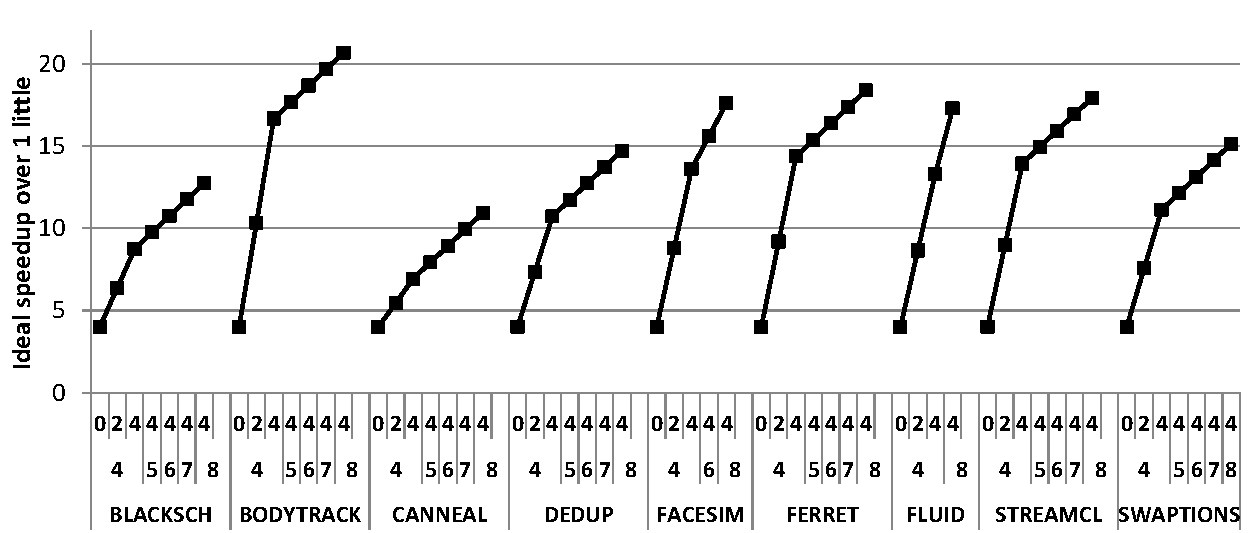
\includegraphics[width=1\columnwidth]{figures/ideal_speedup.pdf}
	\vspace{-0.5cm}
	\caption{Ideal speedup over 1 little core according to Equation~\ref{eq.ideal}. Numbers at the bottom of x axis show the total number of cores, numbers above it show the number of big cores}
	%Results are reported for systems with 0, 2 and 4 big cores, and a total number of cores between 4 and 8.}	
	\label{fig:ideal}%
	\vspace{-0.7cm}
\end{figure}

The original codes make use of the \texttt{pthreads} parallelization model for all the selected benchmarks. The taskified applications follow the same parallelization strategy implemented with OpenMP~4.0 task annotations.
The task-based implementation is done following two basic ideas: i) remove barriers where possible, by adding explicit data-dependencies; and ii) remove application-specific load balancing mechanisms, such as application-specific pools of threads implemented in \texttt{pthreads} and delegate this responsibility to the runtime.
%As a result, both codes achieve the same performance on homogeneous processors with a reduced number of cores~\cite{Chasapis:TACO2016}, while significantly reducing the total number of lines of code for benchmarks with application-specific load balancing mechanisms (bodytrack, dedup and ferret).

%%%%%%%%%%%%%%%%%%%%%%%%%%%%%%%%%%%%%%%%%%
%%%%%%%%%%%%%%%%%%%%%%%%%%%%%%%%%%%%%%%%%%
%\subsection{Performance Ratio Characterization}

When running on the big.LITTLE processor, each benchmark exhibits different performance ratios between big and little cores. These ratios tell us how many times faster a big core is compared to a little core. We measure the performance ratio of each application by executing it first on one big core and then on one little core, which corresponds to Speedup(0, 1, task-based) in Equation~\ref{eq.speedup}. 
% The equation for the performance ratio is the following:
% \begingroup\makeatletter\def\f@size{8}\check@mathfonts
% \begin{equation}
%   \text{Perf\_ratio(workload)} = \frac{\text{Exec. time(workload, 1little)}}{\text{Exec. time(workload, 1big)}}
%   \label{eq.perf_ratio}
% \end{equation}
% \endgroup
Table~\ref{tab:parsec} also includes the observed performance ratio for each application. Bodytrack is the application that benefits the most from running on the big core with a performance ratio of 4.16$\times$. The out-of-order execution of the big core together with an increased number of in-flight instructions significantly improves the performance of this application. In contrast, canneal is the benchmark with the lowest performance ratio, 1.73$\times$, as this is a memory-intensive benchmark that does not benefit as much from the extra computation power of the big core. In general, performance ratios are above 2.5$\times$ for seven out of nine benchmarks, reaching 3.03$\times$ on average. 

% In terms of power, the average ratio is significantly higher, 5$\times$, while the observed values vary between X and Y. \mm{Explain a bit more}.

Taking into account these performance ratios, we can estimate the ideal speedup of the platform for 
each workload assuming a perfect parallelization strategy. Equation \ref{eq.ideal} shows the 
equation for the ideal speedup over 1 little core computation according to the number of big (B) and 
little (L) cores.
\begingroup\makeatletter\def\f@size{8}\check@mathfonts
\begin{equation}
  \text{Ideal speedup(workload, B, L)} = \text{B $\times$ Perf\_ratio(workload) $+$ L}
\label{eq.ideal}
\end{equation}
\endgroup


Figure~\ref{fig:ideal} shows the ideal speedup of the system for each application for the varying 
numbers of cores. This speedup assumes that the applications are fully parallel with no barriers or 
other synchronization points. Thus, these speedups are an upper bound of the achievable application performance.
%As expected, benchmarks with higher performance ratios exhibit potentially higher speed-ups on the asymmetric multi-core.
